\documentclass[english]{article}

\usepackage{babel}
\usepackage{graphicx}
\usepackage{times}
\usepackage{pifont}
\usepackage[margin=1in]{geometry}
\usepackage{eurosym}
\usepackage{fancyhdr}
\usepackage[hidelinks]{hyperref}

\pagestyle{fancy}
\fancyhf{}


%HEADER
%**************************************************************************************
\pagestyle{fancy}
\fancyhf{}
%**************************************************************************************
\lhead{Triggers}		 	 
\rhead{EFP0700 Database Servers} 
\lfoot{EFA12SF}
\cfoot{\thepage}
\rfoot{Alexey Tukalo}
%**************************************************************************************

\date{}
\setlength\parindent{0pt}

\begin{document}

\title{\vspace{2in}Triggers\\
\small for EFP0700 Database Servers\\
\vspace{0.5in}
\includegraphics{savonia.jpg}}

\nopagebreak
\maketitle


\vspace{3in}

\author{
\begin{flushright}
Alexey Tukalo,\\
EFA12SF,\\
Information Technology,\\
Savonia University of Applied Sciences
\end{flushright}
}

\date{\today}
\thispagestyle{empty}

\newpage
\setcounter{page}{1}
\setcounter{tocdepth}{2}
%MAIN CONTENT ******************************************************************************************************************

\section{Introduction}
At the first step I have added the new columns to the tables thought GUI and I also set the default value for user columns via Script below.\\
\centerline{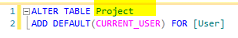
\includegraphics[scale=1]{triggers/Altertables}}\\
To complete all the instructions I decided to write three triggers for every of the three tables. 
\section{The triggers}
\subsection{deleteEmp}
I have started from deleteEmp trigger. The trigger have to prevent any tries to delete row from the table and put the time of the tries into the Removed column on the table. The trigger uses the INSTEAD OF command to fire itself instead of delete command.\\
\centerline{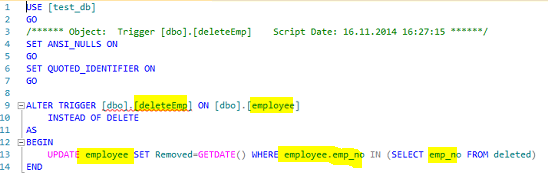
\includegraphics[scale=1]{triggers/deleteEmp}}\\
We also use deleted table to get the reference to the rows which are desired to be deleted.
\subsection{insertEmp}
The trigger has to fill the User and Timestamp columns by current user's name and by current time when new row is created. The trigger is very similar with previous one, but it uses the inserted table, which contain the information about recently inserted row.
\\
\centerline{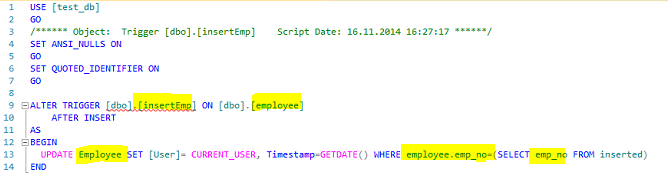
\includegraphics[scale=1]{triggers/insertEmp}}\\
 The trigger should be fired after insert and it is possible to make via command AFTER.

\subsection{updateEmp}
The updateEmp trigger has very same code with insertEmp. It also uses inserted table, because Update actually works like Insert faired after Delete that's why actually in most cases you can use any of the virtual tables.
\\
\centerline{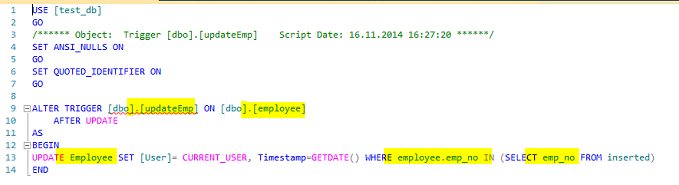
\includegraphics[scale=1]{triggers/updateEmp}}\\

\subsection{Other triggers}
All other triggers can be written via replacing of the triggers names, table names, and primary keys, all the stuff are marked by yellow on the source code of the first three functions.
\\
\centerline{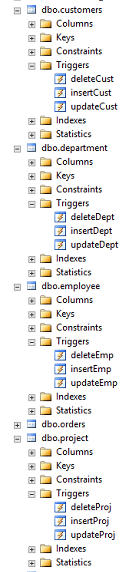
\includegraphics[scale=1]{triggers/struct}}\\
\section{Results}
You can see the results of the work of the triggers on the customers and employee tables bellow.
\\
\\
\centerline{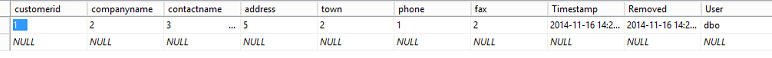
\includegraphics[scale=0.8]{triggers/customers}}\\\\
\centerline{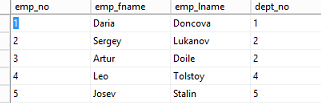
\includegraphics[scale=1]{triggers/employee}}\\




\end{document}
